\subsection{Pivot and Travel Limiter}

\subsubsection{Description}

The pivots main function is to reduce the bending that would be transmitted to the output drive shaft from the drive box and protects the shaft from debris or other objects from coming in contact. The other function of the pivot is to limit the rotation of the exterior drive box to a certain range of rotation. What limits this rotation is a bumper component that is fastened with ten 5/16" bolts to the end of the pivot that is located in the interior of the chassis. This limiter only allows a rotation of 30 degree movement in both directions. The pivot is designed to be able to accept the a 35 mm OD seal,  47 mm tapered roller bearing and a 58 mm OD seal on the end that is fastened to the drive box. Figure~\ref{fig:pivot_assembly_drw} show the final design of the pivot assembly. Do to material limitation, the limiter design wasn't built and installed on the final build. We replaced the limiter with caps to still create the sandwich effect with the flange of the pivot positioned on the outside. Figure~\ref{fig:pivot_bld} show a manufactured pivot.

\begin{figure}[htbp]
\centering
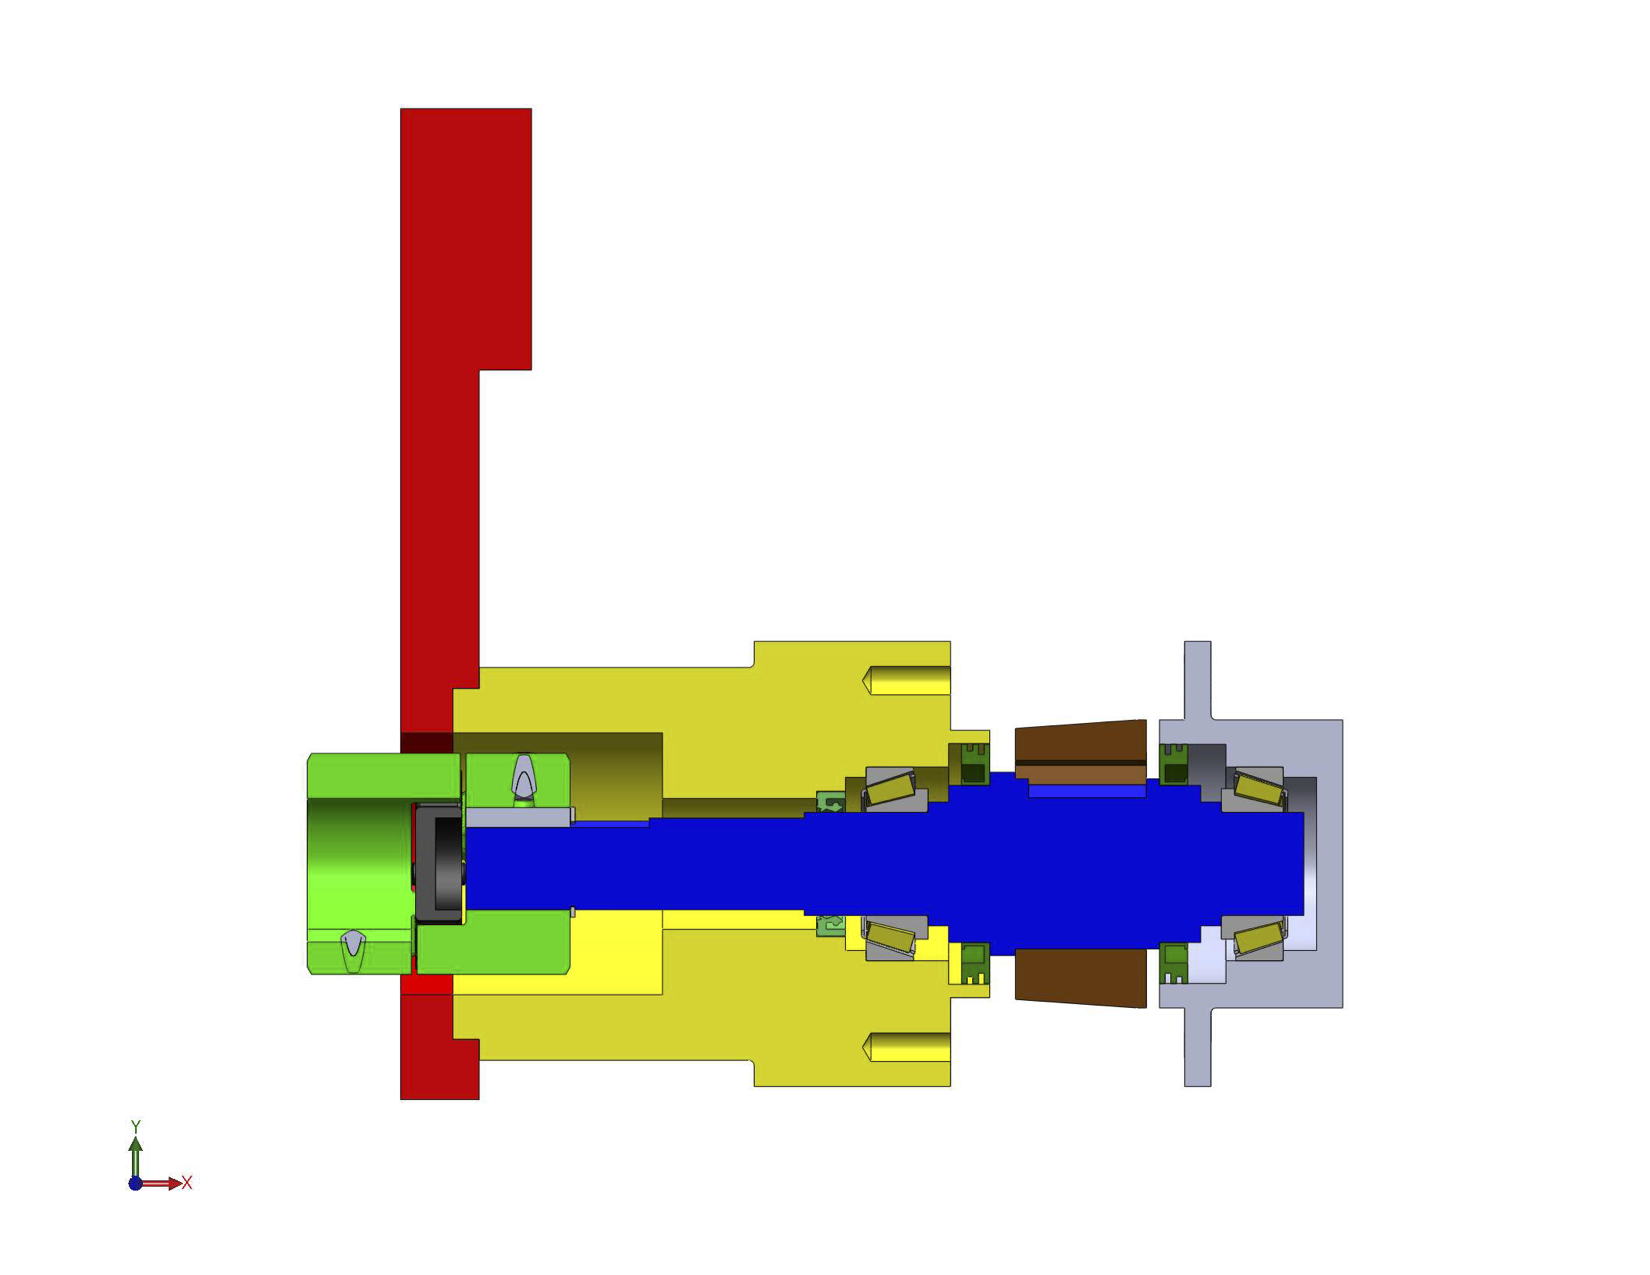
\includegraphics[height=0.3\textheight]{./images/pivot_assembly_drw}
\captionof{figure}[Pivot]{The pivot is shown in yellow and the limiter is shown in red.}
\label{fig:pivot_assembly_drw}
\end{figure}

\begin{figure}[htbp]
\centering
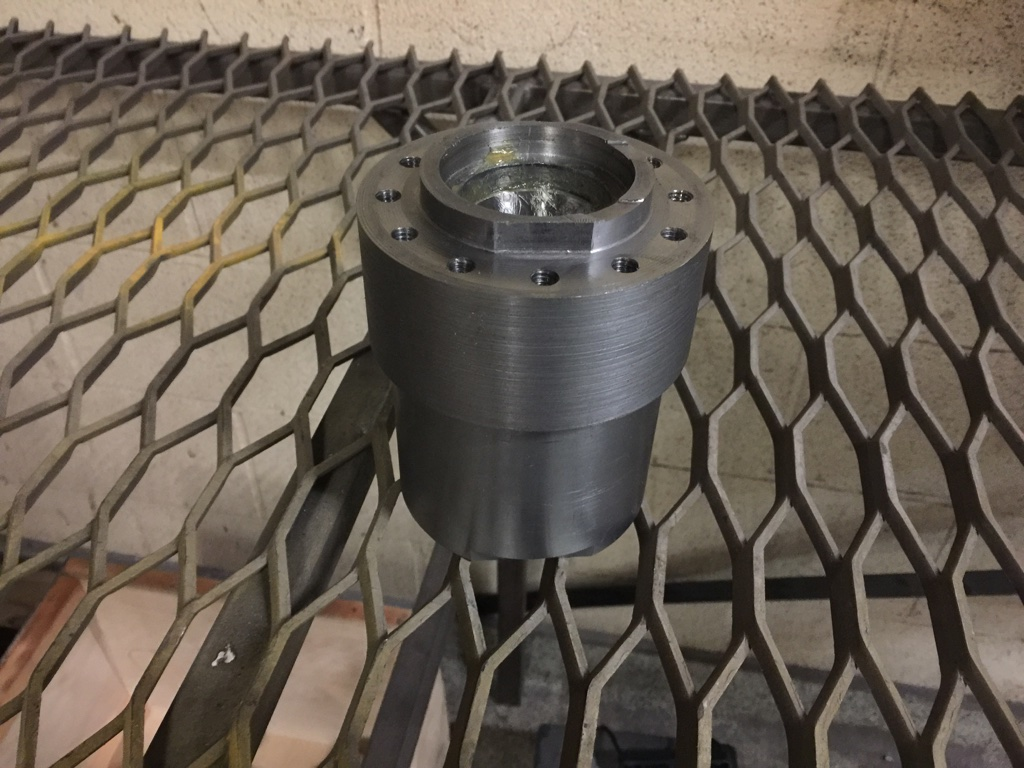
\includegraphics[height=0.3\textheight]{./images/pivot_bld}
\captionof{figure}[Pivot]{Manufactured pivot.}
\label{fig:pivot_bld}
\end{figure}
\newpage



\subsubsection{Design Constraints and Functional Requirements}

The design of the pivot was dimensionally constrained in both its allowable inside and outside diameters as well as the required overhang of the flanged section from the vehicle body. The diameter of the flanged section would also need to be able to accommodate a sufficient number of appropriately sized fasteners for attachment to the drive box, and be sufficiently larger than the pivot body diameter to keep the pivot section axially located against bushings pressed inside the pivot mounting hole in the frame of the vehicle. Additionally, the travel limiter was constrained by the required range of rotation for the pivot, with the travel limiter having flat contact surfaces on both sides. Furthermore, it was necessary for the pivot to remain attached to gear box during assembly and disassembly, with the placement of the pivot to be axially located using two opposing flanges on each of the pivot section and travel limiter. This design would necessitate a simple method of attaching the pivot to the travel limiter to allow for ease of assembly of the drive box to the frame. Table~\ref{tab:pivot_const} outlines the design constraints of the pivot. Finally, the pivot needed to incorporate shoulders to accommodate press fitting the outer race of taper roller bearings and shaft seals inside.



\begin{table}[htbp]
 \centering
 \caption{Pivot Design Constraints and Requirements}
 \begin{tabular}{| p{4cm}llp{6cm} |} \hline
 Constraint & Value & Unit & Reasoning \\ \hline
 Maximum outside diameter & 4 & inch & Constrained by dimensions of frame section available for support \\
 Minimum inside diameter & 2 \textsuperscript{1}/\textsubscript{4} & inch & Chosen to accommodate a coupling to attach drive shaft to driven, output shaft, with a \textsuperscript{1}/\textsubscript{8}'' space between the coupling and the inner wall of the pivot \\
 Length of pivot section outside the vehicle & 1 & inch & To provide spacing between the drive box and the outer frame of the buggy and to accommodate fasteners for drive box attachment \\
 Flange diameter for both pivot and travel limiter & \textsuperscript{1}/\textsubscript{4} & inch & Provide contact surface between flanged face and bushing face. Axial location of pivot within frame mounting section. Bear axial loads applied to pivot during skid steer operation \\
 Angular travel limit for pivot and limiter assembly & 60 & degrees (full range) & Angular range of rotational motion of entire gearbox assembly to prevent contact with upper compartments of frame assembly \\
 Ease of assembly & - & - & General constraint which specifies the need for the pivot section to be attached to the travel limiter, as a two piece assembly, allowing for quick assembly and removal of the gear box \\ \hline
 \end{tabular}
 \label{tab:pivot_const}
 \end{table}
\newpage
The pivot is design to create a pivot point for which the drive box can rotate upon and act a rough suspension. But, the pivot is also design to be compact and bare most, if not all, the stress and strain emitting from the outer drive box during operation. It shouldn't succumb to any plastic bending in either the pivot itself or the bushing and pivot sleeve in the frame insert. Also the limiter should be covered so that no fingers are other body extremities can be pinched during maintenance unless maintenance on the actual limiter. If this is the case, then proper measure should be taken so that no pinching injury happens. The pivot is also design to be modular, as if a section or part of the pivot breaks, replacing the part should be easily managed. 

\subsubsection{Alternate Solution}

A few alternative solutions for the pivot were investigated before a final design was specified. Each design was an iteration of the previous, with modifications made to accommodate the addition of bearings and seals, as well as the accommodation of a removable shaft coupling in more recent iterations. Finite element analysis was performed to determine overall strength of the pivot and was used to reduce the size of the travel limiter.

Figure~\ref{fig:pivotold} and Figure~\ref{fig:pivotfinal} illustrate the intermediate design of both the travel limiter and the final pivot design. It can be seen from the old design that the travel limiter underwent design change where the final design is less complicated to make and was overall a more efficient solution. This version of the design was made with shoulders for a press fit taper roller bearing as well as two shaft seals. The previous iteration of the pivot design saw increases in outer diameter to nearly 4 1/2 ", which was increased to incorporate the addition of taper roller bearings. Again this design was meant to provide shoulders for both shaft seals and bearings, and be able to provide clearance for the drive shaft. Figure and Figure ,illustrate the second design concept. It can be seen that this design made use of twelve 5/16"- 24 bolts to secure the pivot to the drive box. A further ten bolts of the same size were used to fasten the travel limiter to the pivot. The flange diameters for both the travel limiter and the pivot are equal in this design.

\begin{figure}[htbp]
\centering
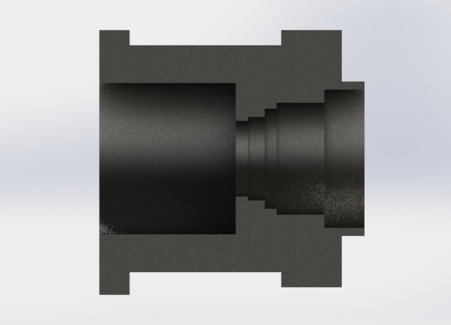
\includegraphics[height=0.3\textheight]{./images/oldpivothaft}
\captionof{figure}[Pivot]{Original pivot design.}
\label{fig:pivotold}
\end{figure}
\newpage
\begin{figure}[htbp]
\centering
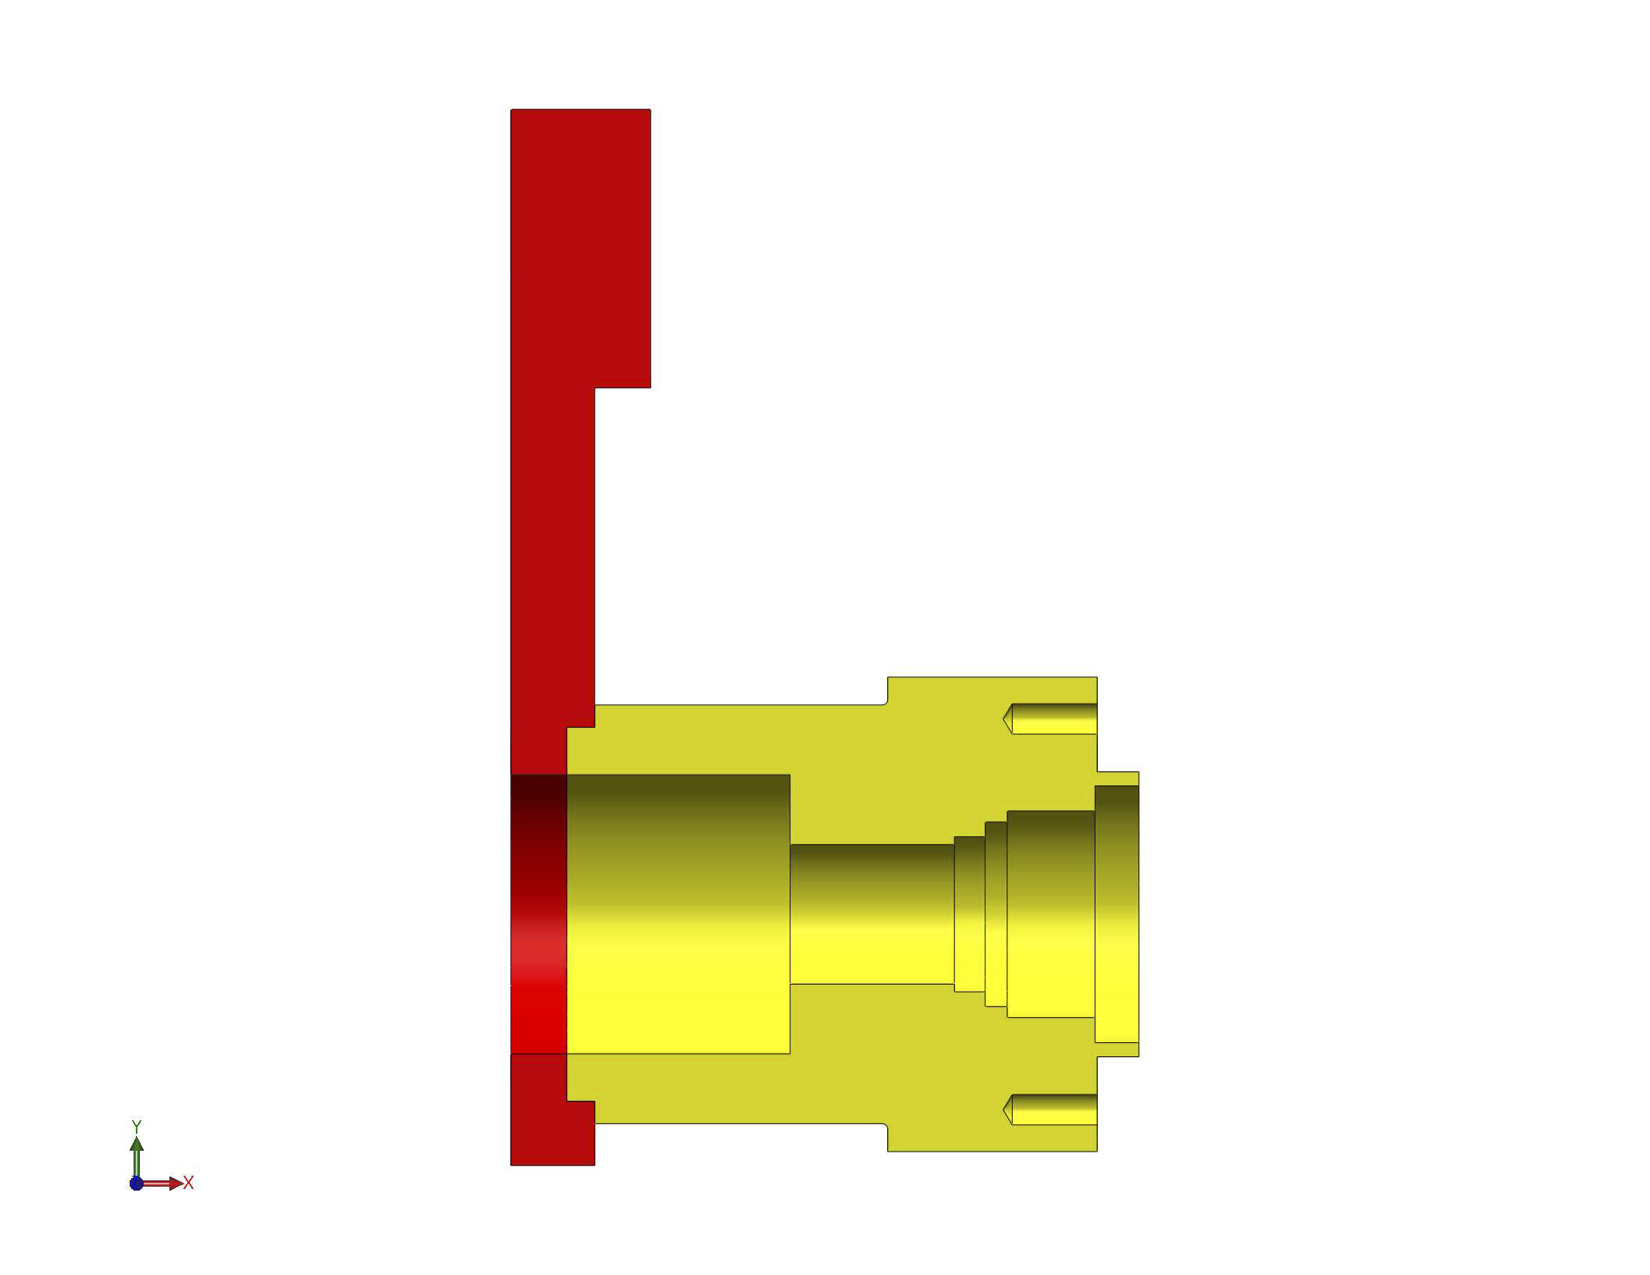
\includegraphics[height=0.3\textheight]{./images/finalpivot}
\captionof{figure}[Pivot]{Final pivot design.}
\label{fig:pivotfinal}
\end{figure}

The final version of the pivot is longer to accommodate the thickness of the pivot sleeve in the frame insert.  Also, in the final pivot design, we reduced the amount of bolt holes for the pivot to drive box connection for the purpose of reducing manufacturing time. We went from 12 to 10 bolt holes and, after bolt calculation, we concluded that having a reduced amount of bolt holes was acceptable while the hole diameter remained the same in both version of the pivots seen above.

\subsubsection{Analysis and Design}

There are four revisions of the pivot that can be seen above in this section. In Appendix~\ref{sec:pivot_fea} of the report, an FEA can be found for each revision. Figure~\ref{fig:pivot_stress_fea} and Figure~\ref{fig:old_pivot_stress_fea} below shows a comparison of the first design of the pivot compared to the final.

%\begin{figure}[htbp]
%\centering
%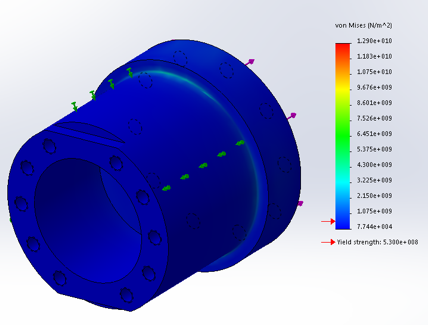
\includegraphics[height=0.3\textheight]{./images/FEA_pivotfinal}
%\captionof{figure}[Pivot]{Von Mises Stresses of final pivot}
%\label{fig:FEA_pivotfinal}
%\end{figure}
%
%\begin{figure}[htbp]
%\centering
%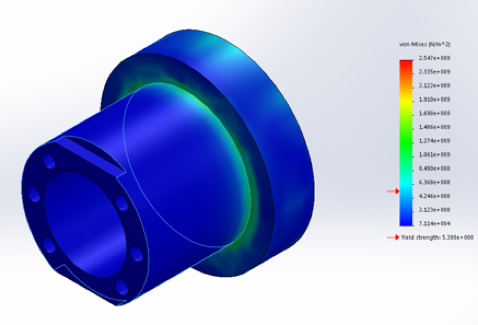
\includegraphics[height=0.3\textheight]{./images/FEA_pivotold}
%\captionof{figure}[Pivot]{Von Mises Stresses of original  pivot.}
%\label{fig:FEA_pivotold}
%\end{figure}

The Von Mises stress maps show the stress concentration around the change in diameter. A fillet was added to reduce the stress concentration in that area. Also the step down diameter was increased to fit the new seal for the taper roller bearing that is located in the pivot. This increase in thickness may also have caused a reduction in the stress experienced.


